\documentclass[11pt,a4paper]{article}

\usepackage{../../templates/style}

\begin{document}

\begin{problem}{นับเลข (Count)}{standard input}{standard output}{1 second}{64 megabytes}

คุณและเพื่อนๆของคุณอีก $n-1$ คน (นับรวมคุณเป็น $n$ คน) นั่งเล่นเกมปัญญาอ่อนด้วยกัน ซึ่งมีกฎดังนี้
\begin{enumerate}

\item ทุกคนจะนั่งกันเป็นวงกลมและจะติดหมายเลขประจำตัวโดยเริ่มจากคนที่ $1, 2, 3, … , n$ (คนที่หมายเลขต่างกัน $1$ จะนั่งติดกันและคนหมายเลข $n$ จะนั่งติดกับคนหมายเลข $1$)

\item เกมจะเริ่มโดยการกำหนดหมายเลข $k$ ขึ้น

\item คนที่มีหมายเลขของตนเป็น $k$ จะต้องลุกออกจากวง จากนั้นคนที่นั่งถัดจากคนหมายเลข $k$ จะต้องเริ่มนับเลข $1$, คนถัดไปนับเลข $2$ ไปเรื่อยๆ (จะไม่นับคนที่ออกจากวงไปแล้ว) จนมีคนนับเลข $k$ ขึ้น กำหนดให้คนที่นับเลข $k$ คือคนหมายเลข i

\item ทำตามข้อ $3$ ซ้ำแต่เปลี่ยนค่า $k$ ให้มีค่าเท่ากับ $i$

\item เกมจะจบเมื่อเหลือคนเพียงคนเดียว ซึ่งก็คือผู้ชนะ
\end{enumerate}

\textbf{ตัวอย่าง} กำหนด $n = 5$ และ $k = 2$

\begin{figure}[h]
\centering
\begin{subfigure}{18ex}
\centering
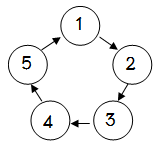
\includegraphics[width=15ex]{../latex/img/1106/1106-1.png}
\end{subfigure}%
\begin{subfigure}{18ex}
\centering
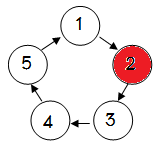
\includegraphics[width=15ex]{../latex/img/1106/1106-2.png}
\end{subfigure}%
\begin{subfigure}{18ex}
\centering
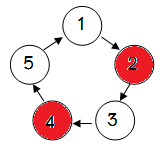
\includegraphics[width=15ex]{../latex/img/1106/1106-3.png}
\end{subfigure}%
\begin{subfigure}{18ex}
\centering
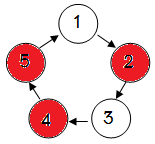
\includegraphics[width=15ex]{../latex/img/1106/1106-4.png}
\end{subfigure}%
\begin{subfigure}{18ex}
\centering
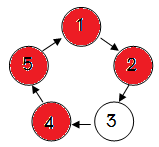
\includegraphics[width=15ex]{../latex/img/1106/1106-5.png}
\end{subfigure}%
\end{figure}

เริ่มต้นที่ $k = 2$ ทำให้หมายเลข $2$ ต้องออกไป (วงกลมสีแดง แสดงถึงหมายเลขที่ออกจากวงไปแล้วและจะไม่เกี่ยวข้องกับเกมอีก)

หลังจากนั้น หมายเลข $3$ จะนับ “1”  หมายเลข $4$ จะนับ “2”  ทำให้ $k = 4$ และหมายเลข $4$ ต้องออกไป

หลังจากนั้น หมายเลข $5$ จะนับ “1”  หมายเลข $1$ จะนับ “2”  หมายเลข $3$ จะนับ “3”  หมายเลข $5$ จะนับ “4”  ทำให้ $k = 5$ และหมายเลข $5$ ต้องออกไป

หลังจากนั้น หมายเลข $1$ จะนับ “1”  หมายเลข $3$ จะนับ “2”  หมายเลข $1$ จะนับ “3”  หมายเลข $3$ จะนับ “4”  หมายเลข $1$ จะนับ “5”  ทำให้ $k = 1$ และหมายเลข $1$ ต้องออกไป

จบการแข่งขัน หมายเลข $3$ เป็นผู้ชนะ

\bigskip
\underline{\textbf{โจทย์}}  กำหนดค่า $n$ และ $k$ จงหาหมายเลขของผู้ชนะ


\InputFile

\textbf{มีบรรทัดเดียว} ประกอบด้วยจำนวนนับ $n$ และ $k$ $( 2 \leq n \leq 200\,000 ; 1 \leq k \leq n )$


\OutputFile

\textbf{มีบรรทัดเดียว} แสดงหมายเลขของผู้ที่ชนะเกมการแข่งขันนี้

\Examples

\begin{example}
\exmp{5 2}{3}%
\exmp{5 3}{4}%
\exmp{5 4}{5}%
\end{example}

  
\Source

สรวิทย์  สุริยกาญจน์ ( PS.int )

ศูนย์ สอวน. โรงเรียนมหิดลวิทยานุสรณ์

\end{problem}

\end{document}